\chapter{Materiales y métodos}\label{chap:materiales}

\section{Contexto y punto de partida}

Este proyecto parte de los datos y de la estrategia de residualización desarrollados en el artículo de referencia
\parencite{bernal2025metabolomics}, pero no se limita a replicar sus resultados. La diferencia principal no está solo en
los algoritmos utilizados, sino en cómo se formula y se recorre el problema. El punto de partida natural es una tarea de
clasificación binaria: para cada paciente se observa un vector de entrada $\mathbf{x} \in \mathbb{R}^p$ y una etiqueta
$y \in \{0,1\}$, donde $y=1$ representa enfermedad de Alzheimer (AD) y $y=0$ control cognitivamente normal (NC). El
objetivo inicial es aprender una función de riesgo

\begin{equation}
f: \mathbb{R}^p \longrightarrow [0,1], \qquad f(\mathbf{x}) = P(y=1\mid\mathbf{x})
\end{equation}

capaz de discriminar entre ambos grupos con capacidad de generalización y un grado de interpretabilidad clínicamente útil.

Ese planteamiento inicial es metodológicamente correcto, pero no agota el problema clínico y, a medida que avanza el
trabajo aparecen dos hechos que obligan a matizarlo. El primero es estadístico: con $N=148$ y una matriz de señal
moderada, la ambigüedad entre clases no desaparece aunque el modelo sea razonable. El segundo es clínico: el coste de un
falso negativo es mayor que el de un falso positivo, por lo que una formulación completamente simétrica del error resulta
ineficiente.

Por ello, el trabajo se estructura en dos fases encadenadas: primero se construye un clasificador metabolómico estable;
después se analiza por qué ese clasificador, aun siendo correcto, no resuelve por sí solo la decisión clínica y debe
reformularse como un problema de triaje con gestión explícita de la incertidumbre.

El artículo de referencia emplea datos de la cohorte TARCC cuantificados con la plataforma Biocrates MxP Quant~500 y
propone una normalización mediante metabolito concomitante para trabajar sobre residuos ajustados por covariables
demográficas. Sobre esa base aplica LDA con validación LOO-CV y explora combinaciones exhaustivas de pocos metabolitos.
El presente TFM hereda la lógica de residualización, de hecho, utiliza una selección representativa de metabolitos
residualizados, pero amplía el análisis en cinco direcciones que son esenciales para la narrativa completa del estudio:

\begin{enumerate}
    \item Incorpora un panel que \textbf{incluye lípidos} además de moléculas pequeñas, lo que cambia sustancialmente la
    firma biológica disponible.
    \item Compara \textbf{familias de modelos} bajo una lectura explícita de sesgo-varianza y tamaño muestral, en lugar
    de aceptar un clasificador por rendimiento aislado.
    \item Utiliza \textbf{stability selection}, \textbf{forward selection} e \textbf{ingeniería de variables} para
    construir un panel parsimonioso y defendible de variables empleadas.
    \item Realiza un \textbf{análisis explícito de errores} para distinguir fallo de modelado de ambigüedad biológica
    real.
    \item Reformula la tarea como un \textbf{sistema de triaje de dos etapas con activación condicional del segundo
    escalón}, donde el bloque clínico-integrador solo interviene cuando el primer nivel no alcanza evidencia suficiente,
    ofreciendo una perspectiva ortogonal al caso de estudio.
\end{enumerate}

La contribución metodológica del trabajo, por tanto, no es únicamente producir un modelo con buen rendimiento, sino
mostrar por qué la secuencia \textit{EDA $\rightarrow$ modelo base $\rightarrow$ límites $\rightarrow$ reformulación
$\rightarrow$ sistema de dos etapas} resulta más fiel al problema real que una clasificación binaria tratada como
objetivo final.

La Figura~\ref{fig:sistema_completo_pipeline} resume de forma sintética todo el flujo aplicado en este TFM, desde la
cohorte de partida y el preprocesado hasta la construcción del modelo de dos etapas y su validación externa.

\begin{figure}[ht]
\centering
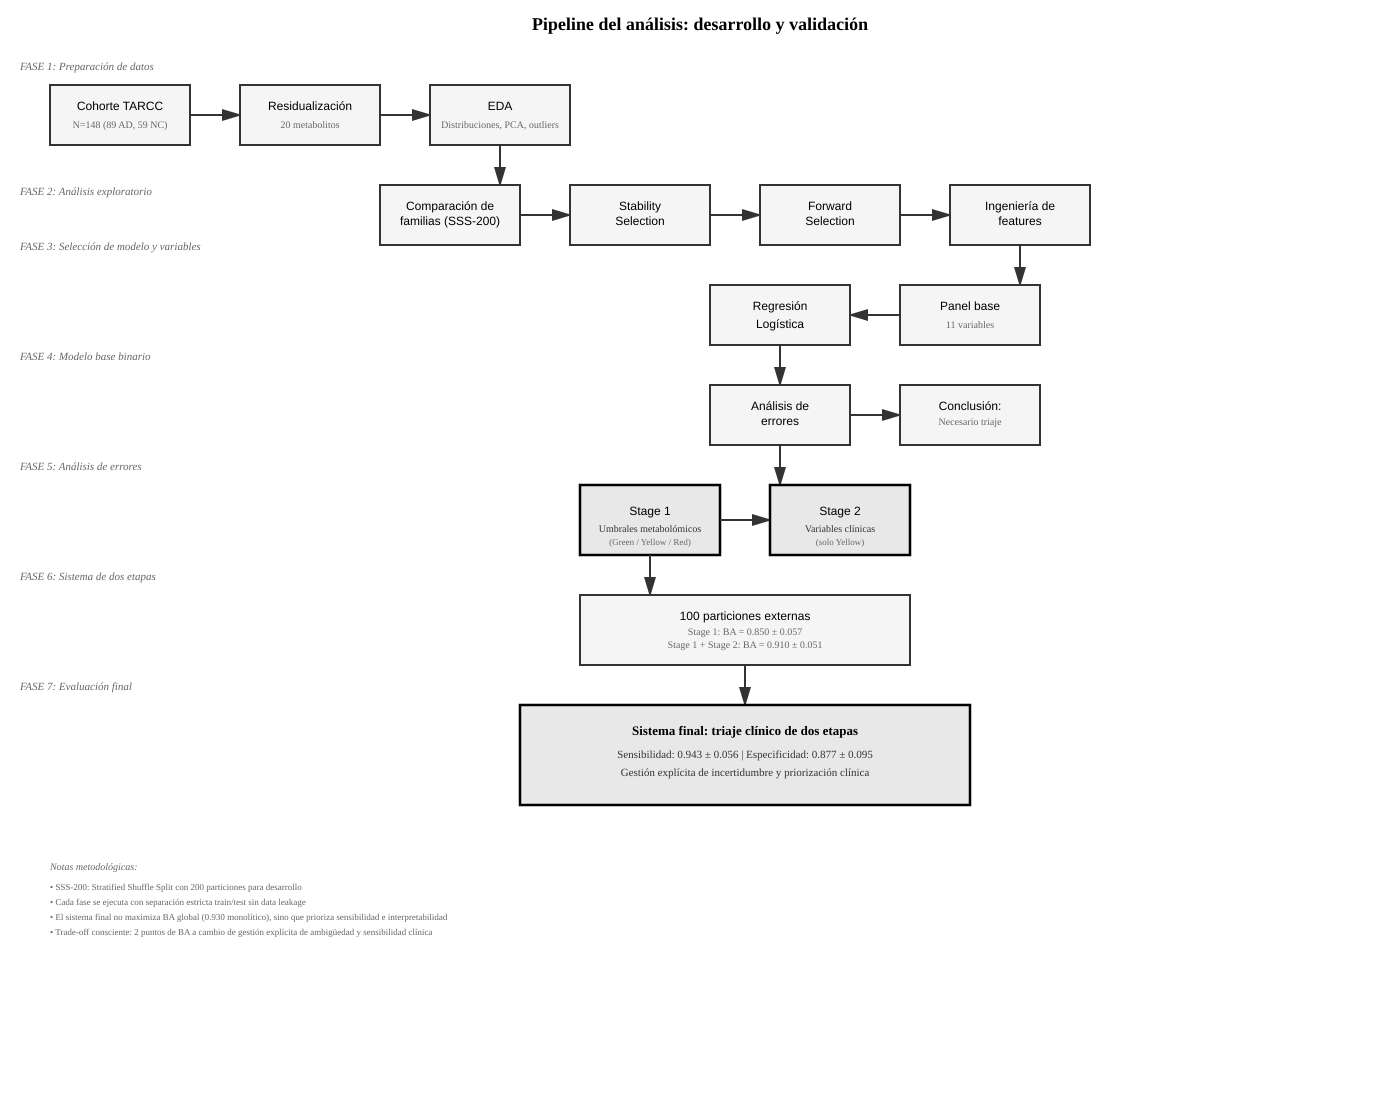
\includegraphics[width=0.92\textwidth]{imagenes/figuras/sistema_completo.png}
\caption{Pipeline completo del sistema propuesto. Se muestran las fases de preparación y selección metabolómica, la transición desde clasificación binaria a triaje clínico en dos etapas y el esquema final de validación externa.}
\label{fig:sistema_completo_pipeline}
\end{figure}

\section{Datos}\label{sec:datos}

\subsection{Cohorte TARCC}

Los datos proceden del \textit{Texas Alzheimer's Research and Care Consortium} (TARCC), un consorcio multicéntrico que
reclutó participantes entre 2005 y 2018 en clínicas de demencia del estado de Texas. Los pacientes AD fueron
diagnosticados según los criterios NINCDS-ADRDA como ``AD probable'', requiriendo consistencia diagnóstica a lo largo de
al menos tres visitas anuales de seguimiento. Los controles son individuos cognitivamente intactos (CDR $= 0$),
reclutados entre familiares y voluntarios.

La matriz final con la que se trabaja en este TFM contiene 148 sujetos: 89 AD y 59 NC. El punto de partida no es el
metaboloma bruto completo, sino el dataset residualizado de 20 metabolitos empleado en el marco del estudio de Bernal et
al., que aquí se adopta como entrada analítica de partida. La diferencia respecto a los 139 casos del artículo no
responde a un cambio conceptual del problema clínico, sino a que allí se aplican filtrados adicionales dentro de
determinadas familias bioquímicas antes de la clasificación, mientras que en este trabajo se parte de esa matriz ya
estabilizada y se preservan todos los sujetos con información útil para el análisis multivariante.

\begin{table}[ht]
\centering
\caption{Características demográficas de la cohorte por grupo diagnóstico.}
\label{tab:demografia}
\begin{tabular}{lcc}
\hline
\textbf{Variable} & \textbf{AD (n=89)} & \textbf{NC (n=59)} \\
\hline
Edad (años), media $\pm$ DE & $71{,}2 \pm 7{,}9$ & $70{,}9 \pm 7{,}7$ \\
Sexo (\% varones) & 48\% & 51\% \\
Tiempo de ayuno (h), media $\pm$ DE & $5{,}8 \pm 4{,}3$ & $4{,}8 \pm 3{,}3$ \\
\hline
\end{tabular}
\end{table}

Edad, sexo y tiempo de ayuno aparecen aquí por dos motivos a la vez. Por un lado, describen el contexto clínico de la
cohorte y por otro, intervienen de manera explícita en la construcción de los residuales. Por eso el análisis posterior
no depende de una comparación inferencial entre grupos en estas covariables, sino de su corrección directa dentro de la
matriz metabolómica de trabajo.

\subsection{Plataforma analítica}\label{sec:biocrates}

La cuantificación se realizó con la plataforma Biocrates MxP\textsuperscript{\textregistered} Quant~500
\parencite{biocrates2020}, que combina cromatografía líquida acoplada a espectrometría de masas en tándem (LC-MS/MS)
para moléculas pequeñas e inyección en flujo con espectrometría de masas (FIA-MS/MS) para especies lipídicas. El panel
completo mide unas 630 señales, entre aminoácidos, aminas biogénicas, ácidos biliares, acilcarnitinas y múltiples
familias de lípidos complejos. Los datos se reportan como áreas integradas, lo que permite comparar sujetos dentro de
cada metabolito, pero no interpretar magnitudes absolutas entre metabolitos distintos como si fuesen concentraciones
equiparables.

Este punto es importante porque condiciona cómo debe construirse la variable de trabajo, debido a que en metabolómica
dirigida, la variabilidad compartida dentro de una familia bioquímica puede reflejar tanto biología de interés como
variación basal del individuo, efectos técnicos o diferencias globales de abundancia; por ello, no basta con llevar las
áreas crudas al clasificador.

\subsection{Construcción de la matriz analítica}\label{sec:matriz_analitica}

La preparación de los datos forma parte, en realidad, de la propia descripción del dataset con el que se trabaja, porque
el modelo no recibe las señales brutas de la plataforma, sino una matriz reducida y transformada para que cada variable
represente la parte verdaderamente informativa del metabolito. Esta descripción se incluye para fijar qué significa cada
variable, no porque en este TFM se reconstruya desde cero el paso desde las aproximadamente 630 señales de la plataforma
hasta los 20 metabolitos residuales: esa matriz ya constituye el punto de partida del análisis.

De forma esquemática, la matriz de partida procede de dos decisiones previas. En primer lugar, el dataset queda
restringido a un subconjunto de 20 metabolitos con señal preliminar y plausibilidad biológica en el contexto AD/NC y,
en segundo lugar, cada uno de esos metabolitos se expresa como residual de una regresión que ajusta por edad, sexo,
tiempo de ayuno y un metabolito concomitante de su misma vecindad bioquímica.

De forma esquemática, para cada sujeto $i$ y metabolito $j$ se trabaja con:

\begin{equation}\label{eq:residuales}
r_{ij} = \log(M_{ij}) - \widehat{\log(M_{ij})}
\end{equation}

donde el término estimado depende de las covariables demográficas y del concomitante correspondiente. Lo relevante aquí
no es el detalle algebraico fino de cada ajuste, sino su interpretación, donde el residual mide cuánto se desvía un
metabolito del nivel esperable para ese individuo una vez descontada la variación basal que comparte con su contexto
metabólico inmediato. Esa es la razón por la que, en lo que sigue, cuando se menciona un metabolito no se está hablando
de su señal bruta, sino de su versión residualizada.

La inclusión del concomitante persigue separar mejor la señal específica del metabolito respecto a la variabilidad común
de su familia, y, del mismo modo, el grupo diagnóstico no entra en la regresión de ajuste, porque hacerlo habría
eliminado precisamente la componente asociada a AD/NC que después se pretende modelar.

El resultado es una matriz sin valores faltantes, centrada alrededor de cero y mucho más adecuada para comparar sujetos
entre sí.

\subsection{Variables del análisis}\label{sec:variables}

Las 20 variables metabolómicas finales se distribuyen en dos bloques, 8 moléculas pequeñas y 12 lípidos. Ese equilibrio
merece destacarse porque se aparta del artículo de referencia, donde los lípidos se descartan en la fase de
clasificación final. Aquí se mantienen porque el análisis parte de una matriz residualizada ya estabilizada y porque el
objetivo metodológico del trabajo exige comparar, sin exclusiones prematuras, distintas familias bioquímicas dentro del
mismo pipeline.

\begin{table}[ht]
\centering
\caption{Metabolitos residuales utilizados como variables de entrada del análisis.}
\label{tab:metabolitos}
\small
\begin{tabular}{lll}
\hline
\textbf{Metabolito} & \textbf{Clase} & \textbf{Papel biológico} \\
\hline
DOPA & Amina biogénica & Precursor dopaminérgico \\
DHEAS & Hormona/esteroide & Neuroesteroide neuroprotector \\
Arg & Aminoácido & Precursor óxido nítrico \\
Spermidine & Poliamina & Autofagia, neuroprotección \\
Ind-SO4 & Indol & Toxina urémica, neuroinflamación \\
HipAcid & Ácido carboxílico & Metabolismo hepático/intestinal \\
GCDCA & Ácido biliar & Eje intestino-cerebro \\
C10:2 & Acilcarnitina & $\beta$-oxidación mitocondrial \\
Cer(d18:1/20:0) & Ceramida & Señalización apoptótica \\
Cer(d18:0/24:1) & Ceramida & Estrés del retículo \\
lysoPC.a.C18:2 & Lisofosfatidilcolina & Inflamación, membrana \\
PC.aa.C40:4 & Fosfatidilcolina & Integridad de membrana \\
DG(16:0\_18:2) & Diacilglicerol & Señalización lipídica \\
TG(18:2\_38:5) & Triglicérido & Metabolismo energético \\
FA(18:2) & Ácido graso & Ácido linoleico (esencial) \\
HexCer(d18:1/26:1) & Hexosilceramida & Metabolismo esfingolipídico \\
Hex2Cer(d18:1/20:0) & Dihexosilceramida & Metabolismo esfingolipídico \\
Hex3Cer(d18:1/24:1) & Trihexosilceramida & Metabolismo esfingolipídico \\
CE(22:5) & Éster de colesterol & Transporte lipídico \\
SM.(OH).C24:1 & Esfingomielina & Mielina, membrana \\
\hline
\end{tabular}
\end{table}

Esta tabla cumple dos funciones. Describe el contenido biológico del panel y, al mismo tiempo, fija el vocabulario del
resto del capítulo. A partir de aquí se hablará de DOPA, Cer20, lysoPC o PC40 como si fueran variables directas, pero
siempre debe entenderse que son residuales ajustados por concomitante y covariables, no concentraciones plasmáticas sin
procesar.

\subsection{Variables clínicas complementarias}\label{sec:variables_clinicas}

Además del bloque metabolómico, se dispone de variables clínicas que no se introducen en el clasificador principal:

\begin{itemize}
    \item \textbf{MMSE} (\textit{Mini-Mental State Examination}): puntuación cognitiva de 0 a 30.
    \item \textbf{APOE}: genotipo de apolipoproteína E (e3/e3, e3/e4, e4/e4).
    \item \textbf{Depresión}: diagnóstico clínico concomitante.
    \item \textbf{Cardiopatía}: comorbilidad cardiovascular considerada en el segundo escalón del sistema.
    \item \textbf{Edad}: covariable demográfica reconsiderada como candidata clínica del segundo escalón.
\end{itemize}

La razón para mantenerlas fuera del modelo metabolómico es, ante todo, conceptual, ya que si se integraran desde el
principio quedaría mucho menos claro qué parte de la señal procede de la firma bioquímica y qué parte responde a
variables clínicas más próximas al fenotipo. Por eso en este capítulo se presentan como variables de segundo escalón y
no como predictores del clasificador binario de referencia.

\section{Análisis exploratorio de datos}\label{sec:eda_metodos}

El análisis exploratorio no se planteó como una descripción ornamental del dataset, sino como el mecanismo que permite
decidir qué clase de modelo resulta defendible y qué pistas aporta de cara a la selección e ingeniería de variables
posterior.
Antes de entrenar ningún clasificador había que responder, al menos, a las siguientes preguntas: si las variables
residuales conservaban una forma regular, si existían outliers capaces de distorsionar la señal, si las escalas eran
comparables, si la dependencia entre metabolitos podía volver inestables los coeficientes, si la separación AD/NC era
real a nivel univariante y, por último, si el tamaño muestral permitía modelos complejos. Las subsecciones siguientes
siguen precisamente ese orden lógico.

\subsection{Panorámica inicial de la matriz analítica}

\begin{table}[ht]
\centering
\caption{Resumen estructural de la matriz usada en el EDA.}
\label{tab:resumen_matriz}
\begin{tabular}{lc}
\hline
\textbf{Característica} & \textbf{Valor} \\
\hline
Sujetos totales & 148 \\
AD & 89 (60,1\%) \\
NC & 59 (39,9\%) \\
Variables metabolómicas & 20 residuales \\
Valores faltantes & 0 \\
Ratio AD:NC & 1,51:1 \\
Ratio $n/p$ & 7,4 \\
EPV (clase minoritaria / variables) & 3,0 \\
\hline
\end{tabular}
\end{table}

Desde el principio aparecen dos restricciones de fondo. La primera es muestral: 20 variables para 148 sujetos es una
relación manejable solo si el modelo se mantiene sobrio y la selección de variables está bien controlada. La segunda es
que el problema no es simétrico, porque la cohorte contiene más AD que NC. De ahí salen dos decisiones de pipeline que
conviene fijar pronto, usar una métrica balanceada en modelado y evaluación \parencite{brodersen2010balanced,powers2011evaluation}, y vigilar con cuidado el coste del
sobreajuste.

\subsection{Forma de las distribuciones y plausibilidad de un modelo lineal}

El interés de esta comprobación es saber si, tras la residualización, las variables conservan una forma aproximadamente
regular, sin asimetrías severas ni colas patológicas que vuelvan inestable cualquier frontera lineal. Si la mayor parte
de los metabolitos residualizados se comporta como una señal continua, centrada y razonablemente simétrica, la hipótesis
de trabajar primero con modelos lineales pasa a ser metodológicamente sensata.

Se evaluó la forma de cada distribución mediante desviación estándar, asimetría, curtosis y test de Shapiro-Wilk.

La lectura empírica de estas comprobaciones se presenta en el capítulo de resultados. En el plano metodológico, lo que
importaba aquí era distinguir entre una matriz todavía demasiado irregular para un modelo lineal y una señal continua lo
bastante estable como para empezar el análisis por familias penalizadas de baja complejidad.

\subsection{Escala y dispersión de las variables}

La homogeneidad de forma no implica homogeneidad de escala, y sabemos que, en un clasificador penalizado, una variable
muy dispersa puede dominar la función de coste aunque su relación con el desenlace no sea más fuerte que la de otra
mucho más compacta. Por eso conviene separar dos cuestiones que a menudo se mezclan: una variable puede ser
aproximadamente normal y, sin embargo, tener una escala incompatible con un ajuste conjunto sin estandarización.

La dispersión de las variables no era homogénea, y ese contraste bastaba para volver inestable cualquier ajuste
penalizado entrenado sobre la escala original. El problema no es solo numérico, sino que, si no se corrige, la
regularización actúa de forma desigual y penaliza más a unas variables que a otras simplemente por cómo están medidas.

La consecuencia metodológica es directa. Desde este punto, cualquier comparación entre modelos y toda selección de
variables debe hacerse sobre datos estandarizados dentro de cada fold, nunca sobre la escala original. No es una
decisión por costumbre: el propio EDA muestra que, sin esa estandarización, la interpretación de los coeficientes y la
estabilidad del modelo quedarían sesgadas desde el inicio.

\subsection{Valores extremos y decisión de winsorizar}

Una vez comprobada la forma global de las distribuciones, el siguiente paso consiste en averiguar si la señal está
dominada por unos pocos sujetos extremos, ya que, en una cohorte pequeña, este punto es especialmente sensible, porque
uno o dos valores atípicos pueden inflar una diferencia entre grupos o, por el contrario, enmascararla si amplían
artificialmente la varianza intragrupo.

Para comprobarlo, se cuantificó la prevalencia de outliers mediante puntuaciones $z$, que es una medida estadística que
indica cuántas desviaciones estándar un punto de datos específico está por encima o por debajo de la media del conjunto
de datos.

\begin{equation}
\qquad Z=(x-\mu)/\sigma
\end{equation}

La decisión de winsorizar no se tomó por rutina, sino como respuesta a este bloque de comprobaciones. Además de contar
la presencia de valores extremos, se estudió si las colas modificaban de forma apreciable la separación univariante entre
AD y NC. La evidencia empírica de ese contraste se presenta en resultados. En términos metodológicos, la consecuencia es
clara, no se eliminaron sujetos, pero sí se decidió winsorizar exclusivamente dentro del entrenamiento de cada split,
sustituyendo los valores por debajo del percentil 5 y por encima del percentil 95 por los propios puntos de corte.

\subsection{Dependencia entre metabolitos y riesgo de multicolinealidad}

Un panel metabolómico no es una colección de variables independientes. Muchas pertenecen a rutas comunes y, si varias
capturan la misma dimensión biológica, un modelo lineal puede repartir sus coeficientes de forma arbitraria. Eso no
siempre empeora la predicción, pero sí vuelve más frágil la interpretación y puede inflar la varianza de los
parámetros cuando $n$ es pequeño.

Para cuantificar ese riesgo se calculó el VIF (\textit{Variance Inflation Factor}):

\begin{equation}
\text{VIF}_j = \frac{1}{1 - R^2_j}
\end{equation}


La intensidad concreta de esas dependencias y su traducción empírica se presentan en resultados. En el plano
metodológico, este bloque justificó dos cautelas, utilizar regularización desde el comienzo y dejar que la selección de
variables resolviera qué parte del panel aportaba señal realmente no redundante.

\subsection{Señal univariante entre AD y NC}

Después de examinar la forma interna del dataset, la pregunta central pasa a ser otra: \textit{¿hay realmente separación
entre grupos?} La forma más directa de responderla es combinar el tamaño del efecto y la significación estadística de
cada metabolito, que, aunque no sirve para decidir el modelo final por sí solo, sí que sirve para saber si el panel
contiene señal biológica o si todo lo que venga después será una construcción artificial del clasificador.

Para hacer visible esa estructura se recurrió, entre otras vistas, a representaciones conjuntas del tamaño del efecto y
de la evidencia estadística. Ese tipo de lectura permite distinguir variables con señal fuerte y robusta, variables con
señal moderada pero plausible y variables prácticamente neutras.

La jerarquía observada de tamaños de efecto, la dirección relativa de los metabolitos principales y la separación visual
entre grupos se presentan en resultados. En términos metodológicos, este bloque cumplía una función concreta, comprobar
si el panel contenía señal biológica real y si esa señal sugería relaciones opuestas o complementarias que justificaran
más adelante una ingeniería limitada de ratios y productos.

\subsection{Tamaño muestral y riesgo de sobreajuste}\label{sec:epv}

El siguiente paso del EDA no describe los datos, sino las limitaciones del estudio. Con demasiada frecuencia se discuten
modelos complejos como si todos fueran opciones igualmente disponibles y solo después se compara cuál rinde mejor. Aquí
esa lógica no era válida, de modo que antes de comparar familias había que comprobar si el problema estaba en un régimen
en el que árboles, kernels o redes neuronales tuviesen alguna posibilidad razonable de generalizar.

\begin{table}[ht]
\centering
\caption{Restricciones muestrales del problema de clasificación.}
\label{tab:restricciones}
\begin{tabular}{lccc}
\hline
\textbf{Métrica} & \textbf{Valor} & \textbf{Umbral recomendado} & \textbf{Lectura} \\
\hline
$n/p$ & 7,4 & $\geq 10$--20 (LogReg) & Ajustado \\
EPV (59/20) & 3,0 & $\geq 10$ & Crítico \\
$n/p$ para RF, MLP o SVM-RBF & 7,4 & $\geq 50$ & Inviable \\
\hline
\end{tabular}
\end{table}

La métrica decisiva es el EPV, que con 59 sujetos en la clase minoritaria y 20 variables, el modelo dispone de unas tres
observaciones informativas por parámetro candidato. Ese régimen no prohíbe técnicamente el ajuste, pero sí vuelve muy
probable que cualquier flexibilidad extra se pague con sobreajuste, por lo tanto, reducir el número de variables no es
una mejora opcional de elegancia estadística, sino que es una condición necesaria para que el problema sea siquiera
abordable con cierta estabilidad.

\subsection{Desbalance de clases y elección de la métrica}

El desbalance de la cohorte es moderado, no extremo, pero aun así, su efecto sobre la evaluación es suficiente para
invalidar la accuracy simple como criterio principal. Un clasificador trivial que etiquetara a todos los sujetos como AD
obtendría un 60,1\% de acierto, pero su especificidad sería nula, por tanto, en un problema cuya utilidad clínica
depende tanto de identificar correctamente a los controles que podrían evitar una LP como de no dejar escapar casos AD,
esa métrica es manifiestamente insuficiente.

\begin{table}[ht]
\centering
\caption{Distribución de clases en la cohorte final.}
\label{tab:clases_eda}
\begin{tabular}{lcc}
\hline
\textbf{Clase} & \textbf{n} & \textbf{Proporción} \\
\hline
AD & 89 & 60,1\% \\
NC & 59 & 39,9\% \\
Ratio AD:NC & \multicolumn{2}{c}{1,51:1} \\
\hline
\end{tabular}
\end{table}

La consecuencia metodológica es doble. Por un lado, el ajuste debe ponderar las clases de forma balanceada para que los
errores en NC no queden infrapenalizados. Por otro, la métrica primaria de comparación será la Balanced Accuracy, que
otorga el mismo peso a sensibilidad y especificidad. Esta decisión no es una preferencia de estilo, sino la única forma
de evitar que el modelo parezca bueno simplemente por alinearse con la clase mayoritaria y de mantener una evaluación
más justa para el caso de uso.

\subsection{Síntesis operativa del EDA}

El EDA no produce todavía un clasificador, pero sí reduce mucho el espacio de soluciones plausibles. De este bloque se
derivaron decisiones muy concretas, empezar por familias lineales, escalar dentro de cada fold, winsorizar en
entrenamiento, vigilar la redundancia entre metabolitos, usar una métrica balanceada y reservar la ingeniería de
variables para relaciones biológicamente defendibles. Con ese marco ya puede formularse una hipótesis de trabajo
razonable, si la señal es real pero moderada, si el tamaño muestral penaliza la complejidad y si varias variables se
organizan en ejes biológicos opuestos, entonces la mejor estrategia debería combinar un modelo lineal regularizado, una
selección de variables explícita y una capa limitada de ingeniería de features bien justificada.

\section{Hipótesis de trabajo}\label{sec:hipotesis}

Del EDA se derivan dos hipótesis formales que guían el resto del análisis:

\begin{description}
    \item[H1 (Parsimonia)] Un modelo lineal regularizado con un subconjunto reducido de metabolitos discriminará AD/NC
     con mejor rendimiento generalizable que cualquier modelo (lineal o no) con las 20 variables,
     debido a las restricciones de EPV documentadas en la Sección~\ref{sec:epv}.

    \item[H2 (Ingeniería de features)] Ratios y productos entre metabolitos con efectos opuestos en AD (fundamentados
    tanto estadística como biológicamente) podrían aportar información discriminativa
    que un modelo lineal no puede extraer de las variables base por separado.
\end{description}

\section{Pipeline de análisis}\label{sec:pipeline}

Esta sección recoge la secuencia operativa que se siguió una vez fijadas las hipótesis del trabajo, es decir, su
objetivo no es solo describir un orden de ejecución, sino dejar claro por qué cada transformación se aplica en ese punto
y qué riesgo metodológico evita. En un estudio con muestra limitada, el pipeline no es una cuestión instrumental menor,
ya que condiciona directamente la validez de la comparación entre modelos, la interpretación de las métricas y la
posibilidad de trasladar el sistema a un escenario de uso real.

\subsection{Prevención de data leakage}

Todo el preprocesamiento se ejecuta estrictamente dentro de cada fold de validación. El procedimiento para cada partición train/test es:

\begin{enumerate}
    \item \textbf{Winsorización en entrenamiento}: se calculan los percentiles 5 y 95 en el training set y se recortan
     únicamente las observaciones del propio entrenamiento que quedan fuera de esos límites. El test set \textbf{no se winsoriza}.
    \item \textbf{Estandarización con \texttt{StandardScaler}}: $z_{ij} = (x_{ij} - \bar{x}_j^{\text{train}}) / s_j^{\text{train}}$. La media y la desviación estándar se estiman exclusivamente en el training set winsorizado.
    \item \textbf{Modelado}: el clasificador se entrena con los datos transformados del training set.
    \item \textbf{Predicción}: el test set se centra y escala con los parámetros aprendidos en training y, sobre esa representación transformada, se generan las predicciones.
\end{enumerate}

Formalmente, para un fold $k$ con índices de entrenamiento $\mathcal{T}_k$ y test $\mathcal{V}_k$:

\begin{align}
\bar{x}_j^{(k)} &= \frac{1}{|\mathcal{T}_k|} \sum_{i \in \mathcal{T}_k} x_{ij} \\
s_j^{(k)} &= \text{std}(\{x_{ij}\}_{i \in \mathcal{T}_k}) \\
z_{ij}^{(k)} &= \frac{x_{ij} - \bar{x}_j^{(k)}}{s_j^{(k)}} \quad \forall i \in \mathcal{T}_k \cup \mathcal{V}_k
\end{align}

Ningún dato del sujeto $i \in \mathcal{V}_k$ participa en el cálculo de $\bar{x}_j^{(k)}$ ni $s_j^{(k)}$. Cuando en el texto se afirma que ``el test set se transforma con los parámetros del training'', esto significa exactamente que la observación de test se proyecta usando la media y la desviación estándar estimadas en el entrenamiento, sin volver a ajustar nada con información del propio test. Esta separación es la condición mínima para evitar \textit{data leakage}.

\subsection{Esquema de validación para desarrollo}

Durante la fase de desarrollo (comparación de familias, selección de variables e incorporación de features construidas), se emplea \textit{Stratified Shuffle Split} con 200 particiones (80\% train, 20\% test, estratificado por clase). Este esquema permite observar cómo cambia el comportamiento del modelo cuando se altera la composición exacta del entrenamiento sin depender de un único corte arbitrario. En cada partición se registran como mínimo BA\textsubscript{train}, BA\textsubscript{test} y AUC\textsubscript{test}; cuando la interpretación clínica lo requiere, también se consideran sensibilidad, especificidad y número de errores.

La métrica primaria de comparación es la Balanced Accuracy en test, porque corrige el desbalance moderado de clases y obliga a vigilar simultáneamente sensibilidad y especificidad. El \textbf{gap de sobreajuste} se define como:

\begin{equation}
\text{Gap} = \text{BA}_{\text{train}} - \text{BA}_{\text{test}}
\end{equation}

Un gap $> 0{,}10$ indica sobreajuste preocupante; gap $< 0{,}02$ es aceptable.

\section{Selección del tipo de modelo}\label{sec:seleccion_modelo}

La selección del clasificador se diseñó como una comparación entre familias, no como una búsqueda ciega del mayor AUC.
La idea fue probar representantes de complejidad distinta para observar su comportamiento bajo las restricciones reales
de esta cohorte, donde el tamaño muestral es limitado, el EPV es crítico y la interpretación probabilística posterior
forma parte del objetivo clínico del trabajo. Por eso cada configuración se evaluó con 200 particiones estratificadas
80/20, registrando de forma sistemática rendimiento en training y test, AUC y gap de sobreajuste.

\subsection{Familia lineal: regresión logística y SVM lineal}

La familia lineal aparecía como la candidata natural tras el EDA, porque si los residuales son regulares, el tamaño
muestral es limitado y la multicolinealidad solo alcanza un nivel moderado, lo esperable es que el mejor compromiso entre
sesgo y varianza aparezca precisamente en este tipo de modelos. La cuestión, por tanto, no era si tenía sentido
evaluarlos, sino con qué grado de regularización convenía hacerlo.

Para ello se utilizó \texttt{GridSearchCV} sobre una malla corta de valores de $C$, entendiendo $C$ como el parámetro que
controla la intensidad de la regularización, donde cuanto menor es $C$, mayor es la penalización y más conservadora
resulta la frontera. En regresión logística se compararon al menos $C \in \{0{,}01, 0{,}1, 1{,}0\}$, mientras que en SVM
lineal se evaluaron configuraciones representativas del mismo orden de magnitud para comprobar si una geometría de
separación distinta aportaba alguna ventaja real.

La comparación empírica entre estas configuraciones se presenta en el capítulo de resultados, donde se analiza cómo
cambia la generalización al relajar la penalización y hasta qué punto el SVM lineal aporta, o no, una geometría de
separación realmente distinta.

\subsection{Familia basada en vecindad: KNN}

Los modelos por vecinos ofrecen una alternativa interesante cuando la relación entre variables y desenlace es local y no
lineal, sin embargo, también son especialmente sensibles al número efectivo de dimensiones y a la geometría de la
muestra. En un espacio de 20 variables con 148 sujetos, la noción de vecindad puede degradarse con rapidez, porque las
distancias entre observaciones se vuelven menos informativas.

Por esa razón se evaluaron varios valores de $k$ como contraste metodológico, no porque KNN fuera la opción preferente a
priori, sino porque ofrecía una referencia útil frente a la familia lineal. Sus resultados se presentan en el capítulo
siguiente junto con la lectura comparativa correspondiente.

\subsection{Familias no lineales de alta capacidad}

El tercer bloque agrupa SVM con kernel RBF, redes neuronales multicapa y ensamblados basados en árboles. Son las
familias que, en principio, podrían capturar interacciones complejas, por eso eran también las más
sospechosas en una cohorte pequeña. Si el EDA estaba en lo cierto, estas familias deberían mostrar rendimientos
aparentes excelentes y generalización pobre.

Precisamente por eso se mantuvieron en la comparación, para comprobar si la flexibilidad adicional abría una región útil
de rendimiento o, por el contrario, entraba demasiado pronto en un régimen de memorización. La evidencia empírica de ese
contraste, junto con su interpretación, se desarrolla en resultados.

\subsection{Síntesis de la comparación y elección del clasificador}

La comparación entre familias se resolvió atendiendo a tres criterios simultáneos, generalización fuera de muestra,
estabilidad probabilística e interpretabilidad suficiente para el uso posterior del modelo dentro del sistema de triaje.
La evidencia empírica de esa comparación se presenta en el capítulo de resultados. A partir de ella, el clasificador de
referencia que se adopta para el bloque binario es una \textbf{regresión logística con penalización L2 y ponderación
balanceada por clase}.

\section{Selección de variables}\label{sec:seleccion_variables}

Una vez fijada la familia del clasificador, el problema central deja de ser qué algoritmo usar y pasa a ser cuánta información puede sostenerse sin desbordar la muestra. El objetivo de esta fase no era reducir por estética, sino comprimir el panel hasta encontrar un punto de equilibrio entre parsimonia, estabilidad y preservación de la señal biológica relevante.

\subsection{Lógica de la selección: robustez primero, recuperación después}

La estrategia se dividió en dos pasos porque ambas tareas responden a preguntas distintas. Primero había que identificar
un núcleo de variables capaz de sostenerse cuando cambia la composición de la muestra y, a partir de ese núcleo,
comprobar si todavía quedaba señal complementaria en metabolitos que por sí solos no alcanzaban plena estabilidad, pero
que sí podían mejorar el conjunto. Este orden importa, porque si se empieza añadiendo variables marginales antes de
asegurar un bloque robusto, la selección tiende a seguir las peculiaridades del split concreto y no la estructura del
problema.

Conceptualmente, la expectativa era sencilla, ya que si la selección estaba bien planteada, el paso de 20 variables a un núcleo
reducido debía recortar el sobreajuste, aunque eso obligara a renunciar a una parte de la señal inicial, y la
recuperación posterior de variables complementarias tenía que devolver parte de esa información sin recrear la fragilidad
del panel completo. Esa lógica se desarrolla de forma gradual en las subsecciones siguientes, en lugar de condensarse por
adelantado en una única tabla global.

\subsection{Stability selection como cribado robusto}\label{sec:stability}

El primer paso fue aplicar \textit{stability selection} siguiendo la lógica de \textcite{meinshausen2010stability}. La
idea es sencilla: una variable verdaderamente informativa debería seguir apareciendo una y otra vez cuando el dataset se
perturba, mientras que una variable oportunista tenderá a desaparecer en cuanto cambie la composición de la muestra.

Operativamente, en cada una de las 200 submuestras estratificadas se ajustó una regresión logística con penalización
L1. Después se registró qué coeficientes quedaban distintos de cero y se calculó su frecuencia de selección:

\begin{equation}
\hat{\Pi}_j = \frac{1}{B} \sum_{b=1}^{B} \mathbb{1}\left[\hat{\beta}_j^{(b)} \neq 0\right]
\end{equation}

Se consideró estable todo metabolito con $\hat{\Pi}_j > 0{,}50$. El umbral no debe leerse como una verdad matemática,
sino como una regla de prudencia fijada para separar un núcleo robusto de un bloque fronterizo, pues obliga a que una
variable demuestre utilidad en más de la mitad de los escenarios muestrales considerados. Este corte se mantuvo fijo en
todo el trabajo y no se reoptimizó a posteriori.

La distribución empírica de frecuencias, el tamaño del núcleo retenido y la posición relativa del bloque fronterizo se
presentan en el capítulo de resultados. Aquí interesa subrayar solo la lógica del procedimiento, primero fijar un bloque
robusto frente a perturbaciones muestrales y, después, decidir si conviene recuperar parte de la señal que ese filtrado
puede dejar fuera.

\subsection{Forward selection para recuperar señal complementaria}

El segundo paso parte de una pregunta concreta: \textit{¿qué variables que no alcanzan plena estabilidad, pero tampoco
son claramente espurias, aportan información adicional cuando se añaden al núcleo robusto?} Para responderla se aplicó
una forward selection competitiva, probando en cada iteración las variables restantes una a una, se añadió la que más
mejoraba la BA y solo se aceptó el cambio si el incremento superaba $\Delta \text{BA} > 0{,}003$. Este umbral debe
leerse como un criterio operativo de entrada mínima y no como una constante óptima del problema.

La forward selection se detiene en cuanto ninguna variable restante supera ese umbral de mejora. Con ello se evita que
el procedimiento siga añadiendo señal débil o dependiente de un único split favorable. La secuencia concreta de
variables recuperadas y el comportamiento empírico de cada paso se presentan en resultados.

\subsection{Lectura conjunta de ambas fases}

La combinación de stability selection y forward selection cumple aquí una función muy precisa. La primera protege frente
a señales dependientes del muestreo y la segunda recupera parte de la información útil que se perdería si el filtrado
robusto se tomara como una frontera absoluta. El resultado empírico de esa secuencia se expone más adelante, pero su
papel metodológico ya queda fijado aquí, construir un bloque de variables base suficientemente estable como para que la
ingeniería posterior no parta de un panel frágil.

\section{Ingeniería de features}\label{sec:feature_engineering}

Un modelo lineal de la forma $\hat{y} = \boldsymbol{\beta}^\top \mathbf{x}$ no puede capturar relaciones multiplicativas
entre variables, ya que si dos metabolitos interactúan biológicamente (por ejemplo, DHEAS como neuroprotector y Cer20 como
pro-apoptótico), su ratio puede ser más informativa que ambos por separado, por lo que la regresión logística no puede
``descubrir'' este ratio, y necesita que se lo proporcionemos explícitamente como feature.

\subsection{Criterio dual de selección}

Las features ingenierizadas se seleccionan por convergencia de dos criterios independientes:

\begin{enumerate}
    \item \textbf{Criterio estadístico} (derivado del EDA):
    \begin{itemize}
        \item Variables con Cohen's $d$ de signos opuestos $\rightarrow$ ratio: si $A$ baja y $B$ sube en AD, $A/B$ es doblemente menor en AD.
        \item Variables con $d$ del mismo signo $\rightarrow$ producto: si $A$ baja y $B$ baja, $A \times B$ captura el ``doble déficit''.
    \end{itemize}

    \item \textbf{Criterio biológico}: cada combinación debe tener interpretación fisiopatológica documentada en el contexto de neurodegeneración.
\end{enumerate}

Que ambos criterios converjan en las mismas combinaciones es lo que distingue este enfoque de un data dredging arbitrario.

\subsection{Features construidas}

Antes de construir ratios e interacciones conviene recordar la lógica del punto de partida. La selección metabolómica
previa deja un bloque de variables base sobre el que se aplican combinaciones candidatas con dos criterios convergentes,
dirección estadística compatible y sentido biológico interpretable. Cuando dos metabolitos se desplazan en sentidos
opuestos, un ratio puede amplificar esa oposición. Cuando ambos lo hacen en la misma dirección, una interacción o un
producto pueden recoger una señal conjunta que el modelo lineal no capta por separado. El orden empírico de esos
metabolitos y el peso relativo de cada uno se presentan en resultados.

\begin{table}[ht]
\centering
\caption{Features ingenierizadas: criterio estadístico y biológico de selección.}
\label{tab:features_eng}
\small
\begin{tabular}{ll>{\raggedright\arraybackslash}p{5cm}>{\raggedright\arraybackslash}p{4cm}}
\hline
\textbf{Feature} & \textbf{Tipo} & \textbf{Criterio estadístico} & \textbf{Interpretación biológica} \\
\hline
$\frac{\text{DHEAS}}{\text{lysoPC.a.C18:2}}$ & Ratio & Desplazamiento opuesto entre neuroesteroide y fosfolípido & Neuroprotección / neuroinflamación \\[6pt]
DOPA $\times$ DHEAS & Producto & Descenso conjunto de dos ejes neurobiológicos & Doble déficit dopamina-esteroide \\[6pt]
PC.aa.C40:4 $\times$ DOPA & Producto & Contraste entre integridad de membrana y neurotransmisión & Desacoplamiento membrana-neurotransmisión \\[6pt]
$\frac{\text{DHEAS}}{\text{Cer(d18:1/20:0)}}$ & Ratio & Oposición entre supervivencia neuronal y señal apoptótica & Supervivencia neuronal / apoptosis \\
\hline
\end{tabular}
\end{table}

\subsection{Incorporación progresiva y validación}

Cada feature se incorporó de forma secuencial y siempre bajo la misma validación SSS-200. El criterio fue simple, una
nueva variable solo podía mantenerse si añadía información verificable fuera de muestra y no convertía la mejora
aparente en una expansión artificial del gap. La trayectoria empírica de esa incorporación, así como la comparación entre
la representación base y la ampliada, se presenta en el capítulo de resultados.

Hasta aquí la lógica del procedimiento es doble. Por una parte, las variables engineered no se añaden por simple deseo
de complejidad, sino porque cada una debe superar un criterio explícito de mejora fuera de muestra. Por otra, una vez
construida la representación ampliada, deja de estar garantizado que todas las variables base sigan siendo igualmente
necesarias. Esa posibilidad obliga a una fase adicional de depuración, que se aborda en la subsección siguiente.


\subsection{Reselección y depuración tras la ingeniería}

La incorporación de variables engineered obliga a revisar si parte de la información de los metabolitos base ha pasado a
estar representada de forma redundante. No se trató de repetir una stability selection completa, sino de aplicar un
procedimiento de depuración funcional sobre el panel ampliado, donde el criterio fue el siguiente: se retiró cada variable base,
de una en una, y se reestimó el modelo completo bajo el mismo esquema SSS-200, de manera que si la retirada de una variable
 no empeoraba la BA\textsubscript{test} y, al mismo tiempo, mantenía o reducía el gap de sobreajuste, esa variable pasaba
 a considerarse candidata a exclusión.

En esta fase, el bloque de partida todavía incluía los metabolitos retenidos por forward selection y las variables
construidas, es decir, una representación ampliada sobre la que se aplicó depuración funcional. Bajo ese criterio se
retiró cada variable base de una en una, reestimando siempre el modelo completo para comprobar si parte de su señal había
pasado a quedar absorbida por las nuevas relaciones entre metabolitos. La secuencia empírica de esa depuración y la
identificación del panel finalmente retenido se presentan en resultados.

\subsection{¿Por qué las features no sustituyen a las bases?}

La ingeniería de variables deja abierta una objeción metodológica razonable. Si las nuevas features solo reexpresaran
información ya contenida en los metabolitos base, entonces su utilidad sería más formal que real. Para comprobarlo se
planificó un análisis de ablación sobre el panel finalmente retenido, eliminando cada feature por separado y reentrenando
el modelo bajo el mismo esquema SSS-200. La evidencia empírica derivada de esa comprobación se presenta en resultados,
pero su función metodológica ya queda definida aquí, distinguir entre una ingeniería meramente decorativa y una
representación que reorganiza información realmente útil.

Un ratio $A/B$ captura la \textit{relación} entre dos metabolitos, pero no sus niveles absolutos. Dos pacientes con la misma ratio pueden tener perfiles biológicos muy distintos:

\begin{equation}
\frac{\text{DHEAS}_1}{\text{Cer20}_1} = \frac{0{,}2}{0{,}4} = 0{,}5 \quad \neq \quad \frac{\text{DHEAS}_2}{\text{Cer20}_2} = \frac{0{,}8}{1{,}6} = 0{,}5
\end{equation}

El modelo necesita ambas informaciones, nivel absoluto en las variables base y relación entre ellas en las features
ingenierizadas. El análisis de ablación descrito en esta sección se diseñó precisamente para comprobar si esas nuevas
variables aportaban información propia o si solo reexpresaban de forma redundante el bloque bioquímico original.

\section{Especificación del clasificador binario}\label{sec:modelo_final}

Una vez definidos el procedimiento de selección, la lógica de ingeniería y la forma de evaluar cada candidato, el paso
siguiente consiste en fijar la especificación del clasificador binario que sirve de referencia para el resto del
trabajo. En este punto no interesa adelantar todavía qué representación concreta acaba reteniéndose, porque esa decisión
pertenece al capítulo de resultados. Aquí basta con dejar establecida la familia del modelo, la forma funcional de la
predicción y el criterio con el que se ajusta su regularización.

\subsection{Forma funcional del clasificador binario}

El bloque de clasificación binaria se formula como una regresión logística regularizada \parencite{cox1958regression,hosmer2000applied} sobre una representación
metabolómica previamente reducida. Esa elección no responde solo a consideraciones de interpretabilidad, sino también a
la necesidad de trabajar con una familia lineal compatible con el tamaño muestral, con el desbalance moderado de clases
y con la presencia esperable de relaciones aproximadamente aditivas tras el preprocesado.

La forma funcional del modelo es:

\begin{equation}\label{eq:modelo}
P(\text{AD} | \mathbf{x}) = \sigma\left(\beta_0 + \sum_{j=1}^{p^\ast} \beta_j \cdot z_j\right), \quad \sigma(t) = \frac{1}{1 + e^{-t}}
\end{equation}

con penalización L2: $\min_{\boldsymbol{\beta}} \left[ -\mathcal{L}(\boldsymbol{\beta}) + \frac{1}{2C} \|\boldsymbol{\beta}\|_2^2 \right]$, donde $\mathcal{L}$ es la log-verosimilitud ponderada por clase.

Aquí $p^\ast$ representa el número de variables retenidas tras la secuencia de selección y depuración descrita en las
secciones anteriores.

En términos de implementación, este clasificador se ajusta como una regresión logística con penalización L2 y
ponderación balanceada de clases. Los parámetros fijos de implementación se mantienen en \texttt{max\_iter=2000} y
\texttt{random\_state=42}, mientras que $C$ queda como hiperparámetro a seleccionar dentro de una malla predefinida.

\subsection{Ajuste de la regularización}

La regularización del clasificador binario no se fijó de forma manual a partir de una sola partición, sino mediante una
búsqueda explícita en rejilla. Una vez fijada la familia del modelo y el procedimiento de selección de variables, el
hiperparámetro realmente decisivo pasa a ser $C$, por lo que se definió una malla logarítmica
$C \in \{0{,}01;\allowbreak 0{,}05;\allowbreak 0{,}1;\allowbreak 0{,}5;\allowbreak 1{,}0;\allowbreak 5{,}0\}$.

La comparación entre valores candidatos se apoyó en dos vistas complementarias. Por un lado, se utilizó
\texttt{GridSearchCV} estratificado sobre el bloque de entrenamiento correspondiente. Por otro, la misma malla se volvió
a examinar dentro de particiones externas repetidas, reestimando siempre winsorización, escalado y ajuste únicamente en
el training set. La evidencia empírica derivada de esa búsqueda, así como la identificación del valor finalmente
retenido, se presenta en el capítulo de resultados.

\section{Validación del clasificador binario}\label{sec:validacion}

La validación se diseñó como un bloque escalonado, porque en una cohorte pequeña la discriminación, la calibración y la utilidad clínica no tienen por qué moverse juntas. Un modelo puede separar bien AD/NC y, aun así, producir probabilidades mal calibradas, depender demasiado del esquema de remuestreo o perder utilidad cuando se traduce a decisiones reales. Por eso se combinaron varios controles, cada uno dirigido a falsar un riesgo metodológico concreto.

\subsection{LOO-CV como validación primaria}

Cada sujeto $i$ se predice con un modelo entrenado en los $n-1 = 147$ restantes:

\begin{equation}
\hat{P}_i(\text{AD}) = f_{\boldsymbol{\theta}^{(-i)}}(\mathbf{x}_i)
\end{equation}

 donde $\boldsymbol{\theta}^{(-i)}$ son los parámetros estimados sin el sujeto $i$. En esta cohorte, LOO-CV no se eligió
 por tradición, sino porque cumple dos funciones simultáneas, por un lado maximiza el tamaño efectivo de entrenamiento
 en cada iteración y produce una probabilidad genuinamente fuera de muestra para cada sujeto, útil para estudiar con
 detalle la distribución de confianza del modelo base.

Las métricas obtenidas bajo este esquema, así como la distribución empírica de probabilidades individuales por grupo
diagnóstico, se presentan en el capítulo de resultados. Aquí interesa únicamente fijar su papel metodológico como
estimación primaria fuera de muestra para cada sujeto.

La limitación conocida de LOO-CV es su varianza relativamente alta, ya que los $n$ folds comparten casi toda la muestra. Precisamente por eso se añadió un bloque de validación complementario que permitiese verificar si las métricas dependían de forma anómala del esquema de remuestreo.

\subsection{Consistencia entre esquemas de remuestreo}

Se aplicó una validación estratificada 10-fold repetida 5 veces (50 evaluaciones), donde la lógica no era sustituir LOO-CV,
sino someterlo a contraste, ya que si ambas estrategias hubieran producido resultados divergentes, eso habría sugerido una
dependencia excesiva de unos pocos sujetos influyentes o de una partición concreta. La comparación empírica entre ambos
esquemas se desarrolla en resultados.
Este contraste cumple dos funciones. En primer lugar, justifica que la estimación basada en LOO no es un artefacto
particular de ese esquema. En segundo lugar, explica por qué en análisis posteriores más costosos, como la evaluación
multi-seed del sistema final de dos etapas, se adopta Repeated Stratified K-Fold (RSKF), ya que ofrece una aproximación
prácticamente equivalente en esta cohorte, pero con un coste computacional menor y una implementación más manejable
cuando el pipeline completo debe repetirse muchas veces.

En esta sección conviene distinguir tres magnitudes distintas. Las métricas \textbf{train} se refieren a rendimiento
estimado dentro del esquema interno de remuestreo; las métricas \textbf{test} proceden del holdout externo reservado; y el \textbf{gap} es la diferencia entre ambas. Esta separación es importante porque un modelo puede tener buena BA de entrenamiento cruzado y, sin embargo, deteriorarse al pasar al holdout final. El gap cuantifica precisamente ese riesgo.

\subsection{Control del optimismo y estabilidad paramétrica}

La siguiente pregunta no es cuánto acierta el modelo, sino cuánto de ese acierto podría ser ilusorio, y para responderla
se comparó el rendimiento aparente, obtenido reentrenando y evaluando sobre toda la cohorte, con el rendimiento validado
por LOO-CV. Ese contraste permite cuantificar el optimismo del ajuste y comprobar si la brecha entre ambos niveles de
rendimiento es compatible con una complejidad bien contenida. La magnitud observada se presenta en resultados.

Ese control se completó con un análisis de estabilidad de coeficientes sobre 200 particiones estratificadas. No bastaba
con que el modelo acertase; importaba también que lo hiciera apoyándose en una estructura razonablemente constante. Para
ello se inspeccionaron signo, dispersión y estabilidad relativa de los coeficientes, utilizando $|\beta|/\mathrm{sd} > 2$
como criterio orientativo de fragilidad potencial.

\subsection{Calibración de probabilidades}

La discriminación no basta para un sistema de triaje. Si el modelo va a derivar o evitar LP en función de umbrales probabilísticos, las probabilidades tienen que ser interpretables en escala clínica \parencite{platt1999probabilistic}. Por eso se evaluó la calibración mediante tres piezas complementarias: Brier score, diagrama de fiabilidad y \textit{Expected Calibration Error} (ECE) \parencite{guo2017calibration}.

El \textbf{Brier score} mide el error cuadrático medio entre probabilidad predicha y desenlace observado; cuanto más
bajo es, mejor es la calibración global. El \textbf{ECE} resume la discrepancia media entre la probabilidad predicha y
la frecuencia real observada en varios intervalos de riesgo, mientras que el primero es una medida global de precisión
probabilística, el segundo ayuda a identificar si las probabilidades están sistemáticamente sobre- o infraestimadas.

Los valores observados de Brier y ECE, junto con el diagrama de fiabilidad correspondiente, se presentan en el capítulo
de resultados. Aquí interesa subrayar solo que la calibración no se trató como una comprobación accesoria, sino como una
condición necesaria para reutilizar la probabilidad del modelo en una lógica posterior de triaje.

\subsection{Robustez clínica y suficiencia muestral}

La validación se extendió, además, a análisis que responden a preguntas translacionales más que algorítmicas. El primer
bloque fue una curva de aprendizaje, para comprobar si el rendimiento seguía creciendo con más datos o si el modelo ya
había agotado la información disponible. Su lectura empírica se presenta en resultados, pero metodológicamente cumple
una función muy concreta: distinguir entre un modelo limitado por mala especificación y un modelo razonable cuya
principal restricción sigue siendo muestral.

El segundo análisis fue una sensibilidad a prevalencia, aquí, resultan especialmente útiles dos métricas:
el \textbf{PPV} ($\mathrm{PPV}=\frac{TP}{TP+FP}$), que indica la probabilidad de que un paciente clasificado como AD lo sea realmente,
 y el \textbf{NPV} ($\mathrm{NPV}=\frac{TN}{TN+FN}$), que mide la fiabilidad de una clasificación negativa. En contextos
  de cribado, donde la prevalencia cambia entre poblaciones, estas dos magnitudes son más informativas que la accuracy
  bruta para entender la utilidad clínica potencial del modelo.

Con ello, la validación deja de ser una colección de métricas aisladas y pasa a cubrir lo que realmente importa en esta
fase del trabajo: discriminación, calibración, estabilidad interna, suficiencia muestral y una primera lectura del
comportamiento del modelo cuando la prevalencia varía.

\section{Diseño del sistema de dos etapas con activación condicional}\label{sec:metodo_cascade}

\subsection{Motivación y cambio de formulación}

El modelo base devuelve una probabilidad $P(\text{AD}) \in [0,1]$ para cada paciente. Esa salida es suficiente para una
clasificación binaria convencional, pero no necesariamente para una decisión clínica cerrada. En este punto del trabajo
la pregunta deja de ser ``qué umbral maximiza una métrica global'' y pasa a ser otra más realista: \textit{si es posible construir un sistema de triaje que resuelva directamente los casos extremos y utilice la información clínica adicional solo cuando la señal metabolómica resulte insuficiente}.

Ese cambio equivale a reformular el problema como una tarea de triaje con costes asimétricos, donde si el coste de un falso
negativo es mayor que el de un falso positivo, entonces el objetivo ya no es optimizar una frontera binaria única, sino
maximizar la cobertura directa del sistema bajo restricciones explícitas de error en las zonas extremas.

La razón por la que las variables clínicas complementarias no se incorporaron desde el principio al modelo metabolómico
es doble. En primer lugar, mezclar ambas fuentes desde el inicio habría dificultado interpretar qué parte del
rendimiento procede de la firma bioquímica y qué parte corresponde a variables clínicas más próximas al fenotipo.
Además, una integración temprana habría mezclado fuentes de evidencia con escalas y funciones distintas dentro de un
mismo ajuste. Por eso se reservan para un segundo escalón, donde aportan contexto solo en la región de ambigüedad.

\subsection{Stage 1: aprendizaje de umbrales de confianza}

Sea $\mathbf{P}_{S1}$ el vector de probabilidades out-of-fold generado por el modelo metabolómico sobre el \textbf{training set} de cada partición externa. En la evaluación definitiva, esas probabilidades se estiman mediante LOO-CV dentro del train, precisamente para que los umbrales se aprendan a partir de predicciones fuera de muestra y no de probabilidades in-sample optimistas. A partir de ese vector se buscan dos umbrales, $t_{lo}$ y $t_{hi}$, que definan tres zonas:

\begin{itemize}
    \item \textbf{Zona verde}: $P < t_{lo}$, casos con evidencia suficiente para clasificación directa como NC.
    \item \textbf{Zona roja}: $P > t_{hi}$, casos con evidencia suficiente para clasificación directa como AD.
    \item \textbf{Zona amarilla}: $t_{lo} \leq P \leq t_{hi}$, casos ambiguos que se derivan al segundo escalón.
\end{itemize}

La selección de umbrales se formula como un problema de cobertura bajo restricción de error:

\begin{equation}
\max_{t_{lo},t_{hi}} \ \mathrm{Coverage}(t_{lo},t_{hi})
\end{equation}

sujeto a

\begin{align}
\mathrm{FN}_{\text{verde}} &= |\{i : P_i < t_{lo} \land y_i = 1\}| \leq \varepsilon_g \\
\mathrm{FP}_{\text{roja}} &= |\{i : P_i > t_{hi} \land y_i = 0\}| \leq \varepsilon_r \\
t_{lo} &< t_{hi}
\end{align}

donde $\varepsilon_g$ y $\varepsilon_r$ controlan la tolerancia de error admisible en cada extremo. En el diseño conservador adoptado en este trabajo, ambos se fijan inicialmente a cero durante el aprendizaje de umbrales sobre probabilidades OOF. La búsqueda es exhaustiva sobre los valores candidatos observados en $\mathbf{P}_{S1}$, por lo que la solución no depende de heurísticas de optimización ni de hiperparámetros adicionales.

Se compararon tres enfoques conceptualmente posibles para definir esas probabilidades de entrenamiento: usar probabilidades
in-sample, usar un esquema LOO y usar un esquema repetido estratificado. El primero se descartó por optimista. LOO se
mantuvo como referencia metodológica para la evaluación final del sistema, mientras que RSKF se conservó como contraste
auxiliar en el análisis del modelo binario base.

Esta formulación es importante por dos motivos. Primero, convierte la incertidumbre en un objeto explícito de diseño: la zona amarilla no es un fallo del sistema, sino una región reconocida de ambigüedad. Segundo, hace que los umbrales sean defendibles en términos clínicos y no solo numéricos.

La rigidez inicial de este diseño, con $\varepsilon_g=0$ y $\varepsilon_r=0$, no se fijó como un dogma, sino como la
versión más conservadora del problema de triaje. La comparación con variantes más tolerantes se presenta en el capítulo
de resultados para comprobar qué cobertura adicional compran y qué coste introducen en términos de error.

\subsection{EDA mínimo del bloque clínico candidato}

Antes de fijar el segundo escalón se revisó el bloque clínico con una lógica deliberadamente más contenida que la del
panel metabolómico. En este punto no se trataba de repetir todo el EDA anterior, sino de comprobar cuatro condiciones
prácticas: disponibilidad suficiente de cada variable en la cohorte, escala y codificación compatibles con un ajuste
conjunto, plausibilidad clínica en el contexto del deterioro cognitivo y complementariedad potencial respecto a la
probabilidad metabolómica generada por el primer escalón.

Bajo ese criterio se inspeccionaron MMSE, APOE, depresión, cardiopatía y edad, prestando especial atención a que ninguna
variable fuese casi constante, a que su codificación mantuviera una lectura clínica razonable y a que el bloque conjunto
no introdujera una redundancia evidente respecto al resumen probabilístico del Stage 1. La evidencia empírica de esta
criba se presenta más adelante; aquí interesa dejar claro que el segundo escalón no nace por acumulación oportunista de
covariables, sino a partir de un bloque pequeño, interpretable y compatible con el tamaño muestral disponible.

\subsection{Construcción y codificación de la entrada clínica}

La entrada del Stage 2 combina la probabilidad $P(\text{AD})_{S1}$ con un pequeño bloque de variables clínicas
complementarias. La matriz candidata de este segundo escalón se construyó a partir de MMSE, APOE, depresión,
cardiopatía y edad, aunque la selección final dentro de ese conjunto se reserva para el capítulo de resultados.

La codificación se diseñó para mantener interpretabilidad y estabilidad. APOE se expresa de forma ordinal según carga de
riesgo, las variables dicotómicas se conservan como indicadores binarios y las variables continuas se integran en el
ajuste con el mismo principio de separación estricta entre entrenamiento y validación que se aplica al bloque
metabolómico.

\subsection{Especificación metodológica del Stage 2}

El segundo escalón no utiliza reglas heurísticas fijas, sino una regresión logística cuya salida se activa únicamente
cuando el caso cae en la subpoblación amarilla. Su función es reinterpretar la probabilidad metabolómica inicial a la
luz de un contexto clínico ortogonal y de bajo número de grados de libertad. La lógica del diseño no es sustituir el
Stage 1, sino complementarlo, porque la primera etapa resume la evidencia bioquímica y la segunda introduce contexto
clínico allí donde esa evidencia no es suficiente para una decisión directa.

En la implementación final, el ajuste del segundo escalón se apoya en el training set completo, incorporando como
variable puente la probabilidad $P(\text{AD})_{S1}$ junto con el bloque clínico. La activación, sin embargo, sí es
condicional: la salida del Stage 2 solo interviene cuando el Stage 1 deja el caso en la zona amarilla.

El modelo adoptado vuelve a ser una regresión logística, ahora con regularización más laxa y ponderación de clases
$\{0:1,1:2\}$. La elección responde al mismo criterio que en el clasificador binario de referencia, mantener un modelo
interpretable, compatible con un número reducido de predictores y alineado con un contexto donde perder un AD sigue
siendo más costoso que sobrediagnosticar un control.

La elección concreta de esa ponderación no debe leerse como una convención arbitraria. Su justificación empírica, junto
con el contraste frente a ponderaciones alternativas, se presenta en el capítulo de resultados.

La regularización del segundo escalón se seleccionó también mediante búsqueda explícita de hiperparámetros. Para ello se
definió una malla logarítmica $C \in \{0{,}01, 0{,}1, 1, 10, 100\}$ sobre la zona amarilla del training, y la comparación
entre valores candidatos se integró después en la evaluación externa repetida del sistema completo. La evidencia empírica
de esa búsqueda, así como la identificación del valor finalmente retenido, se presenta en el capítulo de resultados.

\subsection{Protocolo de evaluación del sistema completo}

La evaluación del sistema respeta estrictamente el flujo de uso real del sistema. Para cada partición externa
train/test:

\begin{enumerate}
    \item se entrena el Stage 1 en train con winsorización y escalado aprendidos únicamente en entrenamiento;
    \item se generan probabilidades out-of-fold en train para aprender $t_{lo}$ y $t_{hi}$;
    \item se entrena el Stage 2 sobre el training set, incorporando $P(\text{AD})_{S1}$ y el bloque clínico, y su salida se reserva para los pacientes que caen en la zona amarilla;
    \item se aplica el sistema completo al test holdout sin recalibrar umbrales ni parámetros con información del propio test.
\end{enumerate}

Este esquema evita dos formas frecuentes de leakage, aprender umbrales sobre probabilidades in-sample y ajustar el
segundo escalón con pacientes cuya información ya ha influido indirectamente en la definición de la zona amarilla.

El Stage 2 no pretende volver a clasificar de forma plana toda la cohorte en la fase de decisión. Su activación está
restringida a la zona amarilla, de modo que los casos verde y roja se resuelven directamente en el primer escalón. Que
el ajuste se realice sobre todo el training set responde a una razón pragmática de estabilidad muestral y no altera la
lógica de uso del sistema, porque la salida del segundo escalón solo interviene cuando el Stage 1 no alcanza evidencia
suficiente.

La evaluación definitiva se realiza con \textbf{100 particiones estratificadas} distintas. Dentro de cada training set,
el Stage 1 genera probabilidades OOF mediante LOO-CV, los umbrales se aprenden sobre esas probabilidades y el Stage 2
se calibra sobre el training set antes de congelar el ajuste final que se aplica al holdout externo. La concordancia
entre LOO-CV y RSKF se examina en el capítulo de resultados, pero el sistema que aquí se reporta corresponde al esquema
interno basado en LOO. Las métricas
primarias del sistema completo son Balanced Accuracy,
sensibilidad, especificidad, número medio de errores y gap train-test. Además, se reportan métricas de train y test del
sistema final, el rendimiento del Stage 1 aislado como baseline, la mejora media aportada por el sistema de dos etapas, la estabilidad
de umbrales y el comportamiento por semilla. En el capítulo de resultados, esta evaluación se complementa con análisis
de persistencia del error por sujeto, comparación pareada entre formulaciones y escenarios de utilidad clínica bajo
distintas prevalencias.

\subsection{Alternativas exploradas y criterio de descarte}

El diseño final no se aceptó por preferencia subjetiva. Se comparó de forma explícita con varias alternativas
plausibles y con mayor sentido metodológico en esta cohorte: ensembles ligeros sobre el Stage 1, stacking con un segundo
modelo complementario, cambios en la regularización del primer escalón y ampliaciones simples del Stage 2. Todas esas
variantes se evaluaron bajo la misma regla metodológica: solo se aceptaría un cambio si
mejoraba de forma consistente la Balanced Accuracy del sistema completo sin aumentar claramente la variabilidad entre
semillas.

Esta regla de aceptación es importante. Evita que una mejora observada en una sola partición o en un experimento local
se convierta en una modificación estructural del sistema. En un estudio con tamaño muestral limitado, la robustez
repetida importa más que la brillantez de un resultado aislado.

\section{Entorno computacional}

El análisis se implementó en Python 3.12, utilizando principalmente \texttt{scikit-learn} para modelado y validación,
\texttt{pandas} y \texttt{numpy} para gestión de datos, \texttt{scipy} para contraste estadístico y
\texttt{matplotlib}/\texttt{seaborn} para visualización.

\subsection{Aplicación interactiva en Streamlit}

Como parte del trabajo se desarrolló una aplicación interactiva en Streamlit que actuó como entorno de exploración,
comparación y validación del pipeline completo. Su valor no es solo instrumental, en un proyecto como este, donde la
interpretación del dato y la comparación iterativa entre alternativas forman parte del propio razonamiento metodológico,
disponer de una interfaz visual e interactiva aporta trazabilidad, reproducibilidad práctica y una lectura mucho más
rápida de los resultados intermedios.

La herramienta se estructuró en páginas especializadas, cada una alineada con una fase del análisis:

\begin{table}[ht]
\centering
\caption{Páginas principales de la aplicación Streamlit y utilidad analítica.}
\label{tab:streamlit_pages}
\begin{tabular}{>{\raggedright\arraybackslash}p{4cm}>{\raggedright\arraybackslash}p{8.5cm}}
\hline
\textbf{Página} & \textbf{Función dentro del análisis} \\
\hline
Exploración de datos & Visualización de distribuciones, outliers, correlaciones, PCA y comparación AD/NC. \\
Selección de variables & Ejecución interactiva de stability selection, forward selection, evaluación incremental e inspección de redundancias. \\
Configuración de modelos & Definición de familias de clasificadores, hiperparámetros y mallas de búsqueda para los modelos base. \\
Evaluación y resultados & Entrenamiento, validación cruzada, métricas en train/test, curvas ROC/PR, matrices de confusión y análisis de calibración. \\
Análisis de errores & Inspección de falsos positivos y falsos negativos, distribución de probabilidades y patrones de alerta. \\
Predicción individual & Aplicación del modelo entrenado a nuevos sujetos y visualización interpretativa de la probabilidad generada. \\
Sistema de dos etapas & Exploración del Stage 1, umbrales de confianza, selección de variables del Stage 2 y evaluación multi-seed del sistema completo. \\
\hline
\end{tabular}
\end{table}

Desde el punto de vista metodológico, esta aplicación resultó útil por cuatro razones. Primero, permitió explorar el EDA
sin depender de scripts estáticos, facilitando la detección de patrones y la comparación de configuraciones.
Segundo, hizo más transparente la selección de variables, porque cada decisión podía visualizarse junto con su efecto
sobre las métricas. Tercero, redujo el riesgo de errores de interpretación al ofrecer un entorno unificado para comparar modelos, esquemas de validación y configuraciones del sistema de dos etapas. Y cuarto, aportó valor de reproducibilidad práctica: el análisis no queda solo como una secuencia de scripts, sino como una herramienta navegable que permite reconstruir el razonamiento seguido en el trabajo.

Además de esta utilidad general, la app permite ejecutar de forma integrada el flujo completo de trabajo: inspección de la cohorte y sus distribuciones; selección de variables por estabilidad, forward y depuración post-ingeniería; configuración explícita del modelo (familia, regularización, pesos de clase y tolerancias); definición del esquema de validación (CV repetida y holdout adicional); análisis detallado de errores por tipo y persistencia; predicción individual con control de umbral de incertidumbre; y exploración del sistema de dos etapas con calibración de umbrales, activación condicional del segundo escalón y evaluación multi-seed.

Las Figuras~\ref{fig:app_streamlit_selection_config} y~\ref{fig:app_streamlit_eval_prediction} muestran cuatro vistas representativas de la herramienta. Estas capturas no pretenden cubrir toda la funcionalidad disponible, pero sí ofrecen una orientación visual suficiente del tipo de interacción y de las decisiones metodológicas que la app permite auditar.

\begin{figure}[!htbp]
\centering
\includegraphics[width=0.49\textwidth]{imagenes/capturas_app/app_01_seleccion_variables.png}
\hfill
\includegraphics[width=0.49\textwidth]{imagenes/capturas_app/app_02_configuracion_modelos.png}
\caption{Vistas de la aplicación para selección de variables y configuración de modelos. A la izquierda se observa el pipeline de selección y el selector manual con métricas asociadas; a la derecha, la parametrización explícita del clasificador y su regularización.}
\label{fig:app_streamlit_selection_config}
\end{figure}

\begin{figure}[!htbp]
\centering
\includegraphics[width=0.49\textwidth]{imagenes/capturas_app/app_03_evaluacion.png}
\hfill
\includegraphics[width=0.49\textwidth]{imagenes/capturas_app/app_04_prediccion_individual.png}
\caption{Vistas de la aplicación para evaluación y predicción individual. A la izquierda se muestra la configuración del protocolo de validación; a la derecha, la interfaz de inferencia por paciente con entrada metabolómica y control del umbral de incertidumbre.}
\label{fig:app_streamlit_eval_prediction}
\end{figure}
